% header
\documentclass[10pt,a4paper]{article}

\usepackage[utf8]{inputenc}
\usepackage{hyperref}
\usepackage{amssymb}
\usepackage{german}
\usepackage{enumitem}
\usepackage{graphicx}
\usepackage{amsmath}
\usepackage{float}

\usepackage{listings} %Quellcodedarstellung

\usepackage{color}
\usepackage{setspace}

%für python code:

\definecolor{Code}{rgb}{0,0,0}
\definecolor{Decorators}{rgb}{0.5,0.5,0.5}
\definecolor{Numbers}{rgb}{0.5,0,0}
\definecolor{MatchingBrackets}{rgb}{0.25,0.5,0.5}
\definecolor{Keywords}{rgb}{0,0,1}
\definecolor{self}{rgb}{0,0,0}
\definecolor{Strings}{rgb}{0,0.63,0}
\definecolor{Comments}{rgb}{0,0.63,1}
\definecolor{Backquotes}{rgb}{0,0,0}
\definecolor{Classname}{rgb}{0,0,0}
\definecolor{FunctionName}{rgb}{0,0,0}
\definecolor{Operators}{rgb}{0,0,0}
\definecolor{Background}{rgb}{0.98,0.98,0.98}

% python umbegung:
\lstnewenvironment{python}[1][]{
\lstset{
numbers=left,
numberstyle=\footnotesize,
numbersep=1em,
xleftmargin=1em,
framextopmargin=2em,
framexbottommargin=2em,
showspaces=false,
showtabs=false,
showstringspaces=false,
frame=l,
tabsize=4,
% Basic
basicstyle=\ttfamily\small\setstretch{1},
backgroundcolor=\color{Background},
language=Python,
% Comments
commentstyle=\color{Comments}\slshape,
% Strings
stringstyle=\color{Strings},
morecomment=[s][\color{Strings}]{"""}{"""},
morecomment=[s][\color{Strings}]{'''}{'''},
% keywords
morekeywords={import,from,class,def,for,while,if,is,in,elif,else,not,and,or,print,break,continue,return,True,False,None,access,as,,del,except,exec,finally,global,import,lambda,pass,print,raise,try,assert},
keywordstyle={\color{Keywords}\bfseries},
% additional keywords
morekeywords={[2]@invariant},
keywordstyle={[2]\color{Decorators}\slshape},
emph={self},
emphstyle={\color{self}\slshape},
%
}}{}



%Das brauchen wir:
\newcommand{\zz}{\mathrm{Z\kern-.3em\raise-0.5ex\hbox{Z}}}

% the document
\begin{document}

% create the title
\title{Klausuraufgaben \\
\small{Kapitel 01}}
\author{The mad physicist}
\date{\today}
\maketitle

\section*{Aufgabe 01}
    \begin{enumerate}[label={\alph*)}]
        \item
            \begin{itemize}
                \item Aufz\"ahlbaum: Ein Baum der alle L\"osungen
                    enth\"alt (?)
                \item Aufz\"ahlungsmethoden: \\
                    \begin{itemize}
                        \item Entscheidungsproblem: 
                            \"Uberpr\"ufe, ob eine 
                            gegebene L\"osung das
                            Problem l\"ost
                        \item Optimierungsproblem:
                            Finde Optimale L\"osung
                    \end{itemize}

            \end{itemize}

        \item Ein Aufz\"ahlungsalgorithmus hei\ss t statisch, wenn der
            Aufz\"ahlungsbaum bereits zu Beginn des Algorithmus vollst\"andig 
            vorliegt. Wird der Baum zur Laufzeit erzeugt, hei\ss t er dynamisch.
    \end{enumerate}
    
\section*{Aufgabe 02}
    \begin{enumerate}[label={\alph*)}]
        
        \item TODO (s. Notizen Seite 7)
        
        \item TODO
        
        \item TODO
        
    \end{enumerate}

\section*{Aufgabe 03}
    TODO (well, that's easy peasy)
    
\section*{Aufgabe 04}
    TODO: diese L\"osung ist nicht ganz so sch\"on!
    
    \begin{python}[frame=single]
def test(field, n, index):
    #teste Reihe und Spalte:
    number = field[index]
    x = index % n
    y = index // n
    for i in range(n):
        if ((field[i*n + x] == number and (i is not y))
            or (field[y*n +i] == number and (i is not x))):
            return False;
    return True

def fill(field,n):
    index = 0
    while (index < n*n and field[index] is not 0):
        index += 1
    if index >= n*n:
        return True
    for i in range(1, n+1):
        field[index] = i
        if test(field, n, index):
            if fill(field, n):
                return True
    field[index] = 0
    return False


def printField(field,n):
    for i in range(n):
        print(field[i*n:(i+1)*n])

# ein Test: (die nullen muessen aufgefuellt werden)
        
testField = [4,0,0,1,0,3,0,0,3,0,1,0,2,1,0,3]

print("Before:")
printField(testField,4)
print("After:")
fill(testField,4)
printField(testField,4)

    \end{python}


\section*{Aufgabe 05}
    \begin{enumerate}[label={\alph*)}]
        \item (TODO: nehme sch\"oneren Pseudocode...)
            \begin{python}[frame=single]
def printField(f):
    for row in f:
        print(row)

def setQueens(fieldQueens, fieldDanger, n, k):
    #print(n)
    if n == k:
        return True
    for x in range(k):
        for y in range(k):
            if fieldDanger[x][y] == 0:
                addQueen(fieldQueens, fieldDanger, k, x, y)
                #printField(fieldQueens)
                #printField(fieldDanger)
                if setQueens(fieldQueens, fieldDanger, n+1, k):
                    return True
                else:
                    removeQueen(fieldQueens, fieldDanger, k, x,y )
    return False

def addQueen(fieldQueens, fieldDanger, k, x, y):
    fieldQueens[x][y] = True
    for i in range(k):
        x0 = x - min(x,y)
        y0 = y - min(x,y)
        if x0+i < k and y0+i < k:
            fieldDanger[(x0+i) % k][(y0+i) % k] += 1
        x0 = x - min(x,k-y-1)
        y0 = y + min(x,k-y-1)
        if x0+i < k and y0 -i >= 0:
            fieldDanger[(x+i)%k][(y+k-i)%k] += 1
        fieldDanger[(x+i)%k][y] += 1
        fieldDanger[x][(y+i)%k] += 1

def removeQueen(fieldQueens, fieldDanger, k, x, y):
    fieldQueens[x][y] = False
    for i in range(k):
        x0 = x - min(x,y)
        y0 = y - min(x,y)
        if x0+i < k and y0+i < k:
            fieldDanger[(x0+i) % k][(y0+i) % k] -= 1
        x0 = x - min(x,k-y-1)
        y0 = y + min(x,k-y-1)
        if x0+i < k and y0 -i >= 0:
            fieldDanger[(x+i)%k][(y+k-i)%k] -= 1
        fieldDanger[(x+i)%k][y] -= 1
        fieldDanger[x][(y+i)%k] -= 1

# ein Beispiel:

if __name__ == "__main__":
    k = 6
    fQ = []
    fD = []
    for i in range(k):
        q_row = []
        d_row = []
        for j in range(k):
            q_row.append(False)
            d_row.append(0)
        fQ.append(q_row)
        fD.append(d_row)

    setQueens(fQ,fD,0,k)

    #gebe aus:
    print("Loesung: ")
    for row in fQ:
        print(row)
            \end{python}
            
            \item diese Teilaufgabe ist wohl trivial...

    \end{enumerate}


\section*{Aufgabe 06}
    TODO (just a long threeliner ...)
    
\section*{Aufgabe 07}
    \begin{enumerate}[label={\alph*)}]
        \item Definition Handlungsreisendenproblem: \\
            Auf einem gerichteten Graphen $G = (V,E)$ mit einer
            Kostenfunktion $c: E \rightarrow \mathbb{R}$
            sollen alle Knoten in $V$ 
            besucht werden. Es soll die L\"osung mit minimalen Kosten
            gefunden werden.
        \item Betrachte Graph: \\
            \begin{figure}[H]
                \centering
                \def\svgwidth{\columnwidth}
                \resizebox{0.5\textwidth}{!}{
                    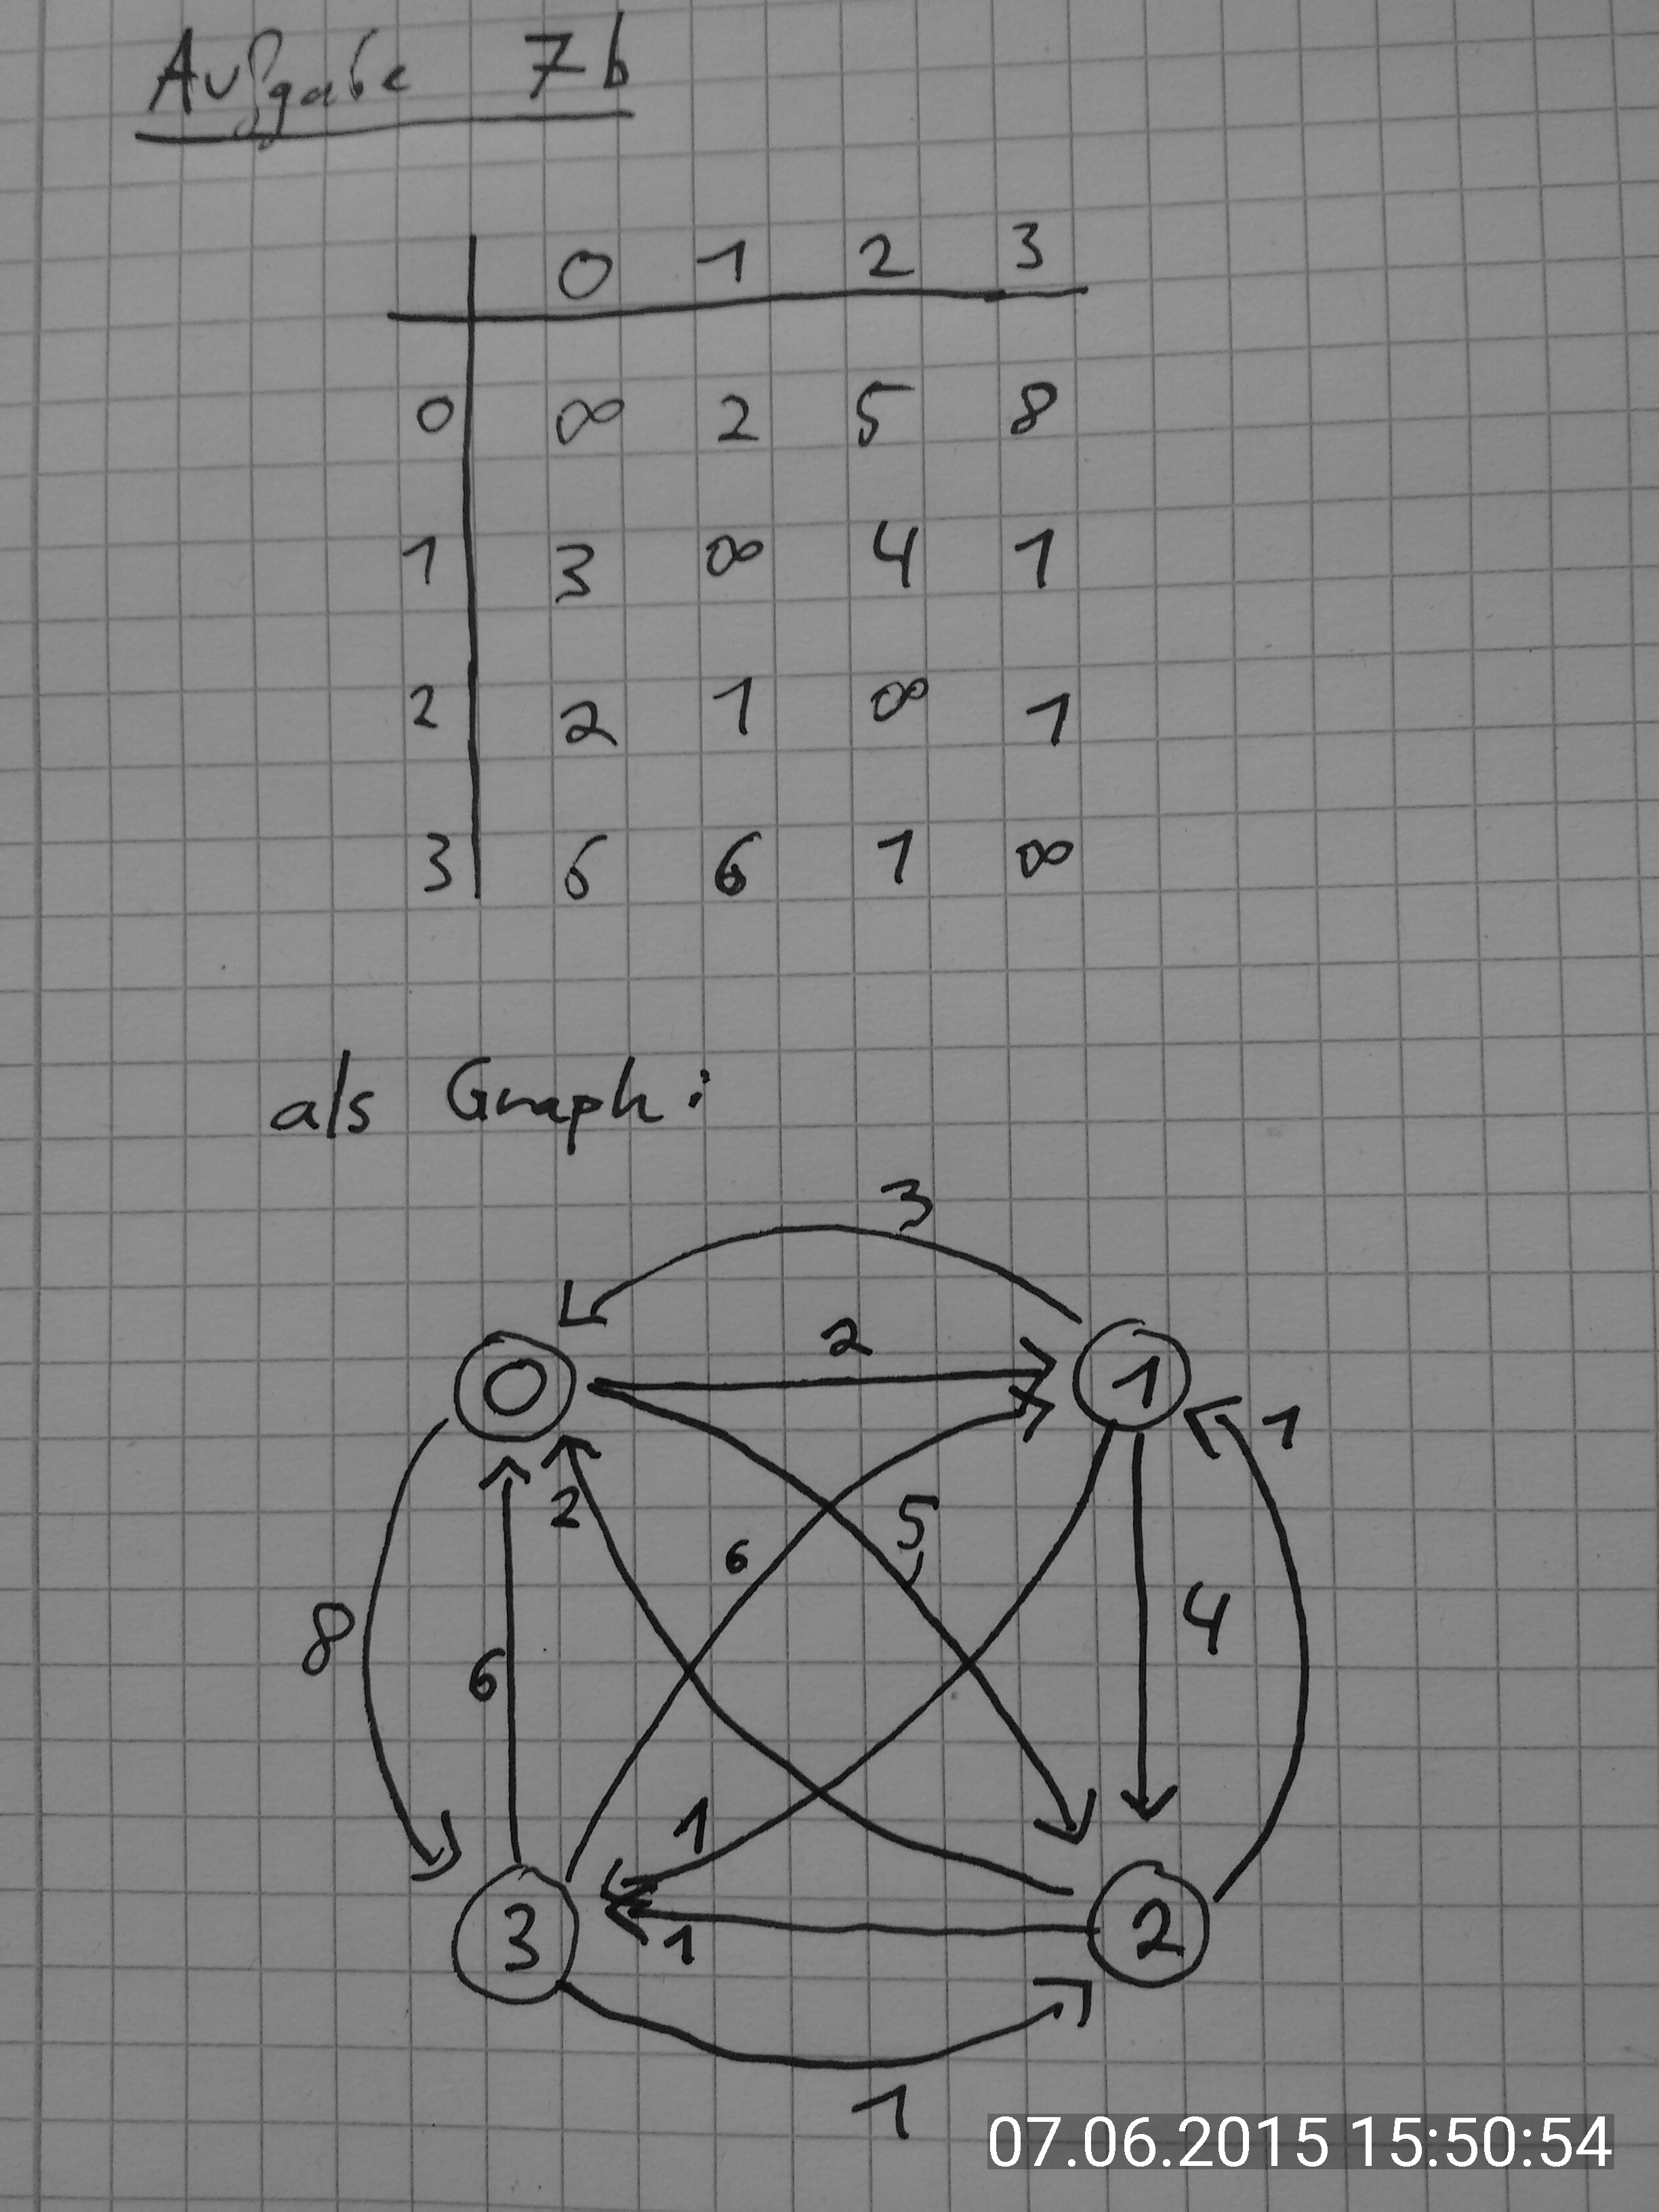
\includegraphics{01_07b1.jpg}
                }
            \end{figure}
            Die minimalen Kosten betragen nach s. 10 des Skripts:
            $$
                c_0 = 0.5 \cdot \sum_{i=0}^{n-1} 
                \left( \min\limits_{j \neq i} c(j,i) + 
                \min\limits_{l \neq i} c(i,l) \right)
            $$
            Das ist in unserem Fall:
            $$
                c_0 = \frac{1}{2} \cdot 
                    ((2+2)+(1+1)+(1+1)+(1+1))
                    = 5
            $$
            \begin{figure}[H]
                \centering
                \def\svgwidth{\columnwidth}
                \resizebox{0.5\textwidth}{!}{
                    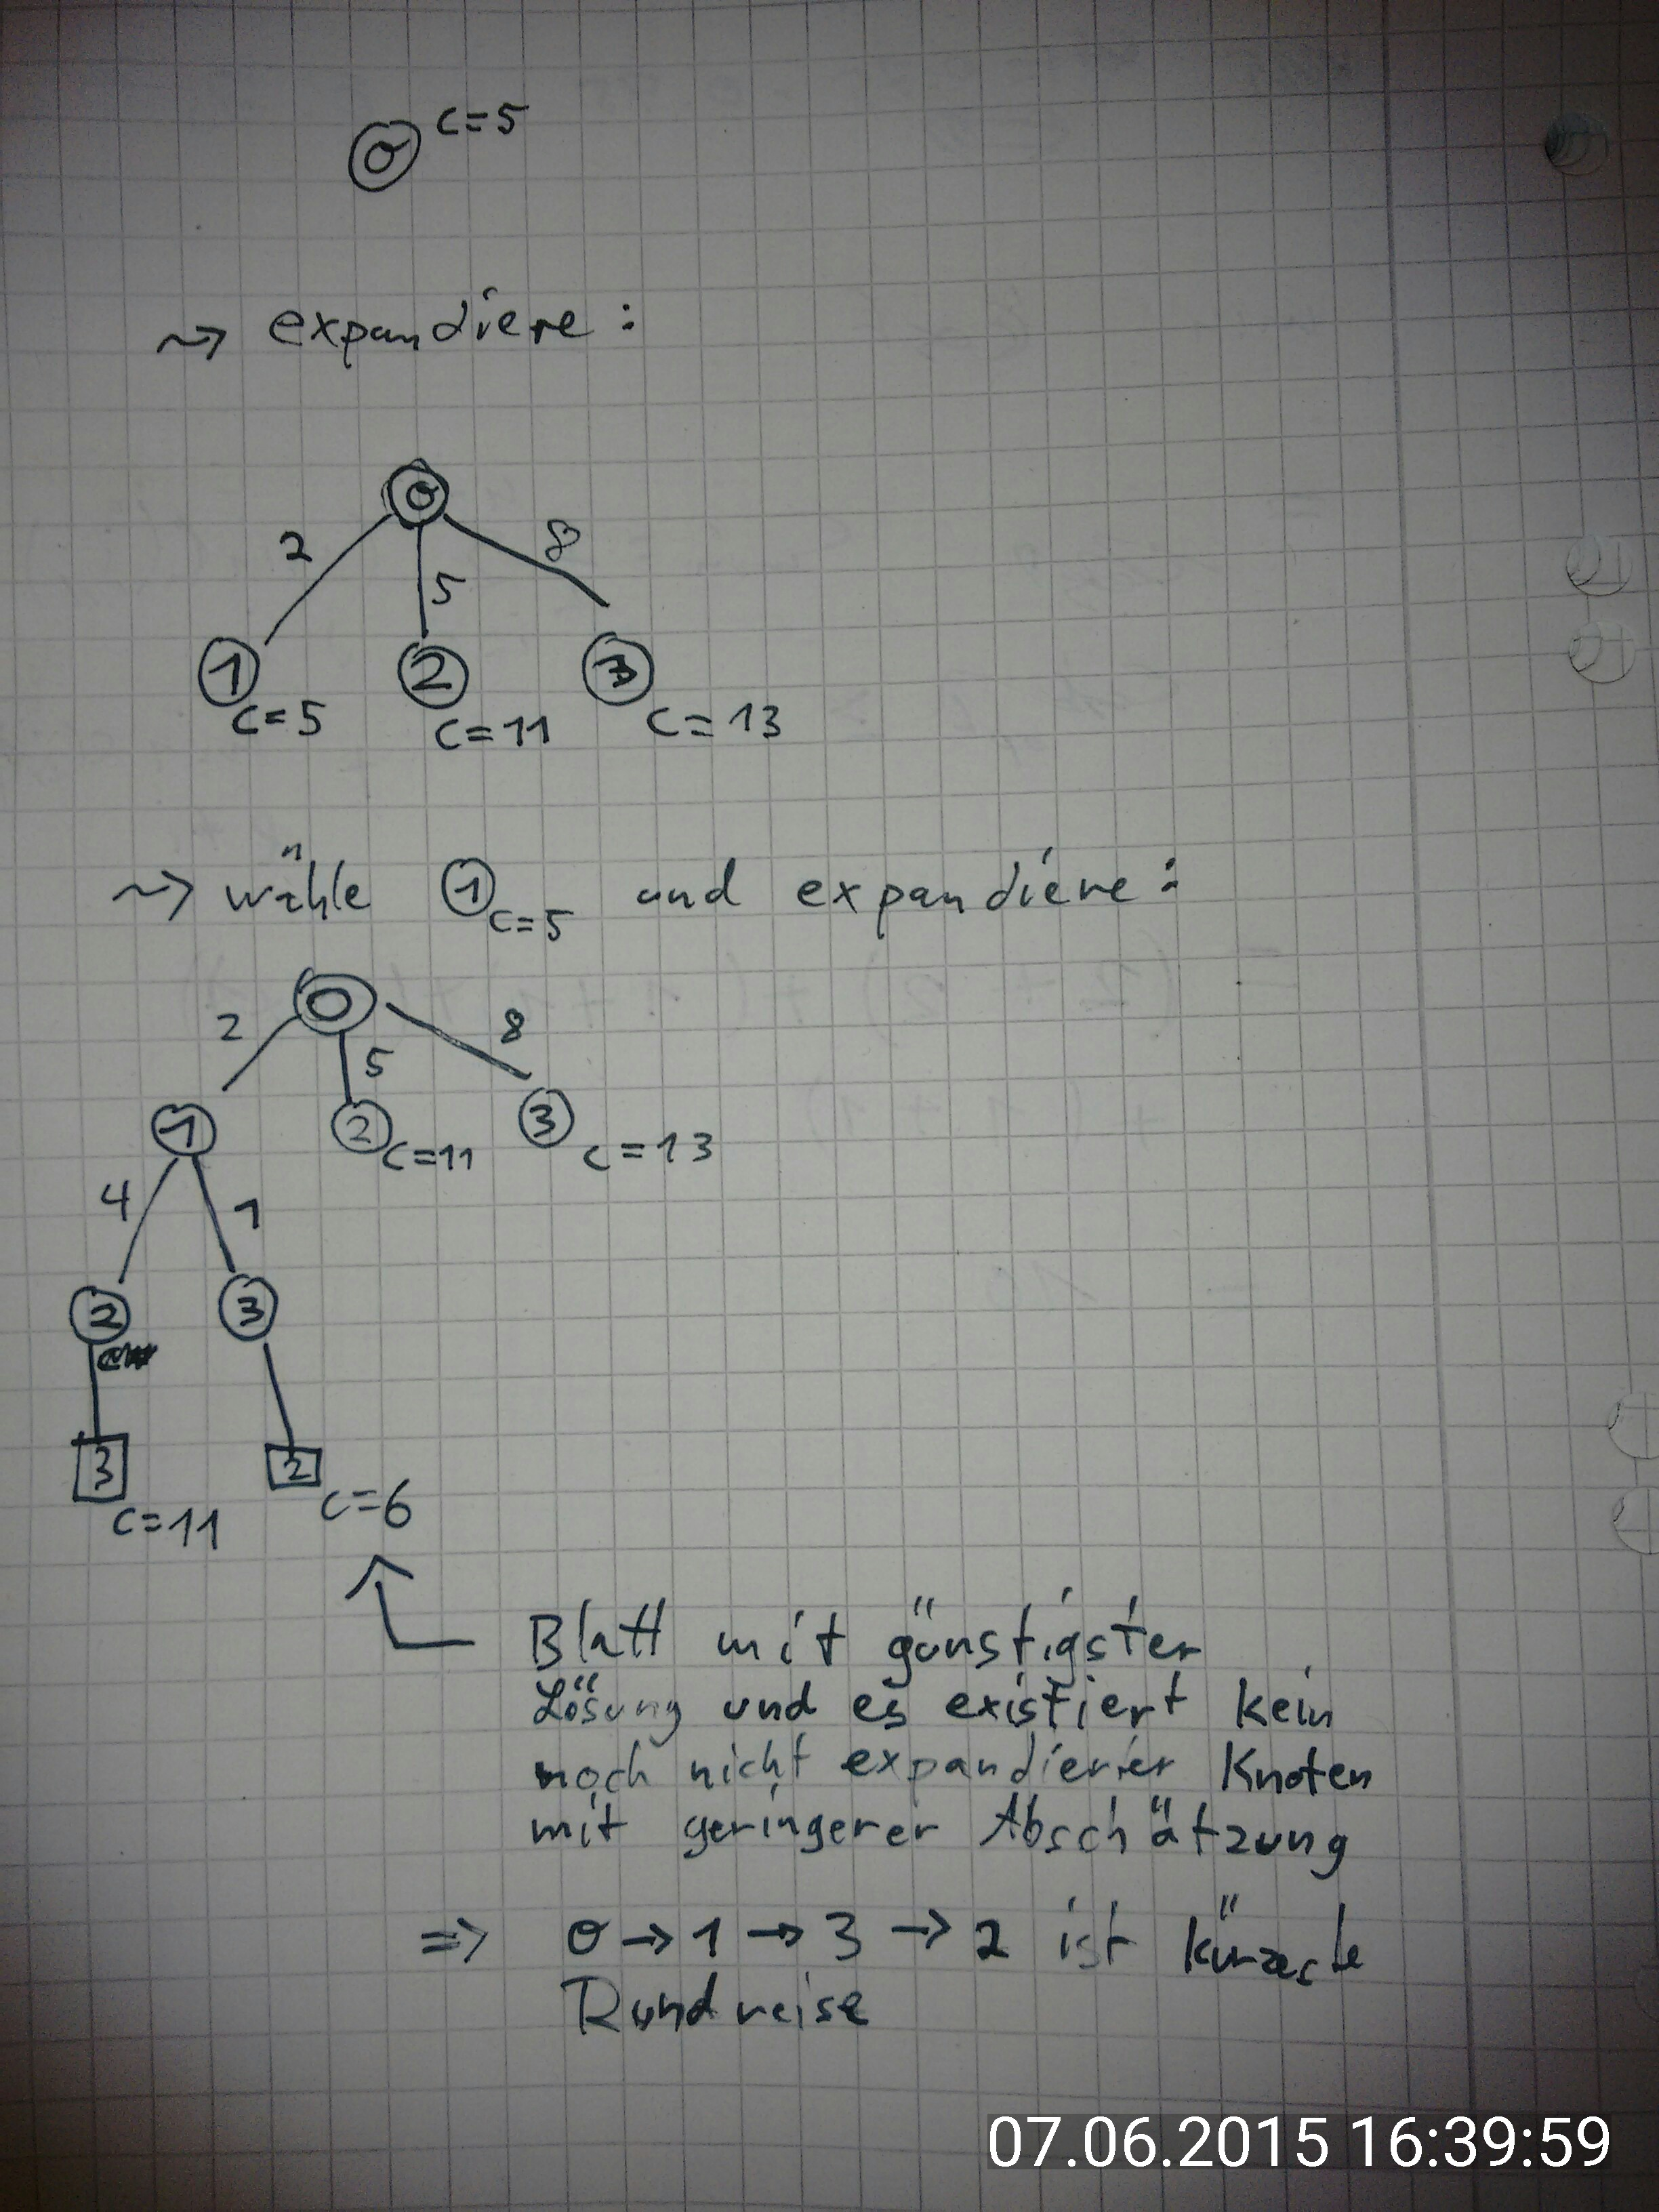
\includegraphics{01_07b2.jpg}
                }
            \end{figure}
            (TODO: Matrizen f\"ur jeden Iterationsschritt fehlen!)
            
    \end{enumerate}

    
\section*{Aufgabe 08}
    Seien ${p_1, p_2, \ldots, p_n}$ die Personen, die die Br\"ucke \"uberqueren
    sollen. Die Kosten f\"ur einen Lauf zur anderen Seite der Personen seien
    $c_1, c_2, \ldots, c_n$. Sei $c_{1st}$ die Kosten der schnellsten Person
    f\"ur einen Lauf und $c_{2nd}$ die Kosten der zweitschnellsten Person 
    f\"ur einen Lauf. Dann k\"onnen wir die Zeit nach unten hin absch\"atzen mit:
    $$
        c_{min} = (n-1) \cdot c_{2nd} + (n-2) \cdot c_{1st}
    $$
    (Anm: $\mathbf{(n-1) \cdot c_{2nd}}$ f\"ur die ``Hinwege'', 
    $\mathbf{(n-2) \cdot c_{1st}}$ f\"ur die ``R\"uckwege'') \\
    Um uns die Sache einfacher zu machen, definieren wir uns einen Knoten
    im Aufz\"ahlungsbaum als Zustand und speichern daher auch alle
    Werte, die wir zum Aufz\"ahlen des Knotens brauchen in denselben.
    Die Kosten des Knotens werden durch $c(v)$ mit $v \in V$ beschrieben
    (Keine Ahnung, wie das im Skript genau definiert ist, deshalb schreibe ich
    es hier noch mal hin; Gez. Jonas).
    Desweiteren definieren wir LS (f\"ur linke Seite) als die Start-, 
    und RS als die Endseite der Br\"ucke.
    Ein Knoten hat als Attribute die Mengen L (mit den Personen auf der
    linken Seite) und R (mit den Personen auf der Rechten Seite).
    und die Iterationstiefe i. Ein Iterationsschritt (= einer Kante von einem
    Knoten v nach v') besteht aus zwei Schritten:
    \begin{itemize}
        \item Die Person in v.R mit minimalen Kosten l\"auft mit der Lampe nach
              v'.L (wir gehen ohne Beweis davon aus, dass diese Strategie immer
              zu keinem schlechteren Resultat als andere Aktionen f\"uhren)
        \item Zwei Personen aus v.R laufen nach v'.L 
    \end{itemize}
    Daraus resultieren f\"ur v' folgende Attribute:
    \begin{itemize}
        \item v'.i = v.i + 1
        \item v'.L und v'.R ergeben sich aus der obigen Beschreibung
    \end{itemize}
    Bleiben noch die Kosten f\"ur v' zu aktualisieren. Dabei sei $c_{1st_r}$ in diesem
    Kontext die Kosten der schnellsten Person aus v'.R und $c_{1st_l}$ die Kosten
    der schnellsten Person aus v'.L . Dann gilt:
    
    $$
        c(v') = v + (n-v.i-1) \cdot c_{1st_l} + (n-v.i-2) \cdot c_{1st_r}
    $$
    
    nun l\"asst sich das Problem mit der Kostenfunktion c(v) f\"ur jeden
    Knoten v ganz normal mit branch and bound l\"osen.


    
    
\section*{Aufgabe 09}
    \begin{enumerate}[label={\alph*)}]
        \item Handlungsreisendenproblem mit Dreiecksungleichung ($\Delta HR$): \\
            gegeben ist:
            \begin{itemize}
                \item $G = (V,E)$
                \item $V = \left\{0,1,\ldots, n-1\right\}$
                \item $c: E \rightarrow \mathbb{N}_0 $ mit:
                    \begin{itemize}
                        \item $c(i,j) = c(j,i) \forall i,j \in V$ (Symmetrie)
                        \item $c(i,j) \leq c(i,k) + c(k,j)$ (Dreiecksungleichung)
                    \end{itemize}

            \end{itemize}

            
    \end{enumerate}

    
\section*{Aufgabe 10}
    TODO
    
\section*{Aufgabe 11}
    TODO
    
\section*{Aufgabe 12}
    TODO
    
\section*{Aufgabe 13}
    TODO
    
    
    



\end{document}